\documentclass[aps,pra,twocolumn,superscriptaddress,nofootinbib,longbibliography,floatfix]{revtex4-2}
\usepackage[T1]{fontenc}
\usepackage[utf8]{inputenc}
\usepackage{amsmath,amssymb,amsthm}
\usepackage{booktabs}
\usepackage{graphicx}
\usepackage{xcolor}
\usepackage[hidelinks]{hyperref}

% The author block for both manuscripts. OWNER-SET ONLY.
%
% The name, affiliation and contact on a paper are statements the author
% makes. Set by the owner on 2026-09-14 ("Josh Philbrick"); the affiliation
% and contact are the ones his public profile and earlier public release
% (Ariadne, 2026-06-08) already use. `build.py --release` refuses while any
% placeholder remains.
\newcommand{\OwnerAuthor}{\author{Josh Philbrick}\email{Josh@coherenceenergylabs.com}}
\newcommand{\OwnerAffiliation}{\affiliation{Coherence Energy Labs}}
\newcommand{\OwnerEmail}{Josh@coherenceenergylabs.com}

% GENERATED by paper/tools/make_numbers.py from evidence/ -- do not edit.
% Every value below is read from an artifact at generation time.
\newcommand{\AuditAccepted}{1{,}588}
\newcommand{\AuditEpsMax}{\ensuremath{2.6\times 10^{-13}}}
\newcommand{\AuditExactSame}{842}
\newcommand{\AuditExactSamePct}{53}
\newcommand{\AuditHeadProducer}{1{,}197}
\newcommand{\AuditInadmissible}{0}
\newcommand{\AuditOracleEqual}{1{,}352}
\newcommand{\AuditOracleMaxDelta}{\ensuremath{2.7\times 10^{-15}}}
\newcommand{\AuditOracleN}{1{,}399}
\newcommand{\AuditRuleTerm}{\ensuremath{1.4\times 10^{-7}}}
\newcommand{\CertifyMsPerShot}{106.34}
\newcommand{\CheckExponent}{1.076}
\newcommand{\CheckRSquared}{0.995}
\newcommand{\CheckSupportExponent}{0.86}
\newcommand{\CheckWorkExponent}{0.58}
\newcommand{\ConfRefusals}{48}
\newcommand{\ConfVectors}{56}
\newcommand{\ConfVectorsMinusOne}{55}
\newcommand{\CostRatioBatch}{6{,}610}
\newcommand{\CostRatioPerShot}{3{,}591}
\newcommand{\DecodeUsBatch}{16}
\newcommand{\DecodeUsPerShot}{30}
\newcommand{\DetCleanFalseAlarms}{1}
\newcommand{\DetCleanFalseAlarmsFull}{0}
\newcommand{\DetCleanN}{770}
\newcommand{\DetCleanPymAboveEps}{0}
\newcommand{\DetCleanPymExcessPositive}{14}
\newcommand{\DetControlFlagged}{0}
\newcommand{\DetControlN}{62}
\newcommand{\DetDefectAll}{4{,}862}
\newcommand{\DetDefectInvalid}{3{,}549}
\newcommand{\DetDefectN}{4{,}861}
\newcommand{\DetDefectNonDefective}{1}
\newcommand{\DetDefectNonDefectiveFlagged}{0}
\newcommand{\DetDefectNotProven}{0}
\newcommand{\DetDefectProven}{1{,}312}
\newcommand{\DetStaleControlFalseAlarms}{1}
\newcommand{\DetStaleControlSuboptimal}{0}
\newcommand{\DetStaleCorrections}{6{,}147}
\newcommand{\DetStaleDThreeBoth}{6}
\newcommand{\DetStaleDThreeProven}{24}
\newcommand{\DetStaleDThreeStaleErrors}{7}
\newcommand{\DetStaleDThreeStaleOnly}{1}
\newcommand{\DetStaleDThreeTrueErrors}{7}
\newcommand{\DetStaleDThreeTrueOnly}{1}
\newcommand{\DetStaleExcessHiOneFive}{0.25}
\newcommand{\DetStaleExcessHiThree}{0.64}
\newcommand{\DetStaleExcessLoOneFive}{0.13}
\newcommand{\DetStaleExcessLoThree}{0.39}
\newcommand{\DetStaleFalseAlarms}{2}
\newcommand{\DetStaleProven}{547}
\newcommand{\DetStaleSuboptimal}{547}
\newcommand{\DetStaleSuboptimalOneFive}{110}
\newcommand{\DetStaleSuboptimalThree}{271}
\newcommand{\DetStaleSuboptimalTwo}{166}
\newcommand{\DetStealthN}{1{,}312}
\newcommand{\DetStealthProven}{1{,}312}
\newcommand{\EpsBoundaryInsideAccepted}{\textbf{[pending]}}
\newcommand{\EpsBoundaryRefused}{\textbf{[pending]}}
\newcommand{\EpsFewerConfigs}{\textbf{[pending]}}
\newcommand{\EpsForgeriesTotal}{\textbf{[pending]}}
\newcommand{\EpsHwAccepted}{\textbf{[pending]}}
\newcommand{\EpsHwAcceptedPct}{\textbf{[pending]}}
\newcommand{\EpsHwExact}{\textbf{[pending]}}
\newcommand{\EpsHwForgeries}{\textbf{[pending]}}
\newcommand{\EpsHwGenFourPct}{\textbf{[pending]}}
\newcommand{\EpsHwGenSixPct}{\textbf{[pending]}}
\newcommand{\EpsHwLargestEps}{\textbf{[pending]}}
\newcommand{\EpsHwNontrivial}{\textbf{[pending]}}
\newcommand{\EpsHwNotProven}{\textbf{[pending]}}
\newcommand{\EpsLargestEps}{\textbf{[pending]}}
\newcommand{\EpsMoreConfigs}{\textbf{[pending]}}
\newcommand{\EpsSimAccepted}{998{,}145}
\newcommand{\EpsSimAcceptedPct}{99.81}
\newcommand{\EpsSimChunkRetries}{0}
\newcommand{\EpsSimExact}{8{,}628}
\newcommand{\EpsSimForgeries}{8{,}000{,}001}
\newcommand{\EpsSimForgeryClasses}{9}
\newcommand{\EpsSimLargestEps}{\ensuremath{6.2\times 10^{-12}}}
\newcommand{\EpsSimNontrivial}{1{,}000{,}000}
\newcommand{\EpsSimNotProven}{1{,}855}
\newcommand{\EpsSimNotProvenPct}{0.19}
\newcommand{\EpsSimShots}{1{,}000{,}000}
\newcommand{\EpsSubstitutedRefused}{\textbf{[pending]}}
\newcommand{\FaultCorpus}{4{,}924}
\newcommand{\FaultsAll}{4{,}861}
\newcommand{\FaultsAllCertCaught}{4{,}861}
\newcommand{\FaultsAllSyndromeCaught}{3{,}549}
\newcommand{\FaultsAllSyndromePct}{73.0}
\newcommand{\FaultsControl}{62}
\newcommand{\FaultsControlFlagged}{0}
\newcommand{\FaultsStealth}{1{,}312}
\newcommand{\FaultsStealthCertCaught}{1{,}312}
\newcommand{\FaultsStealthSyndromeCaught}{0}
\newcommand{\GapBmPNinetyNine}{1.5 / 3.0 / 4.9}
\newcommand{\GapBposdExactHi}{81}
\newcommand{\GapBposdExactLo}{72}
\newcommand{\GapBposdMax}{148}
\newcommand{\GapBposdPNinetyNine}{38 / 61 / 52}
\newcommand{\GapExactRuleBposdExact}{81.5 / 72.3 / 77.1}
\newcommand{\GapExactRuleCertified}{227 / 383 / 253}
\newcommand{\GapShotsPerDistance}{400}
\newcommand{\GrowthDSevenCertified}{31/120}
\newcommand{\GrowthSpeedupHi}{64}
\newcommand{\GrowthSpeedupLo}{17}
\newcommand{\HwCoreSecX}{3.87}
\newcommand{\HwCoreSecZ}{3.48}
\newcommand{\HwFinalCertified}{198{,}770}
\newcommand{\HwFinalGenFourCertified}{98{,}772}
\newcommand{\HwFinalGenFourNontrivial}{99{,}384}
\newcommand{\HwFinalGenFourPct}{99.38}
\newcommand{\HwFinalGenSixCertified}{99{,}998}
\newcommand{\HwFinalGenSixNontrivial}{100{,}000}
\newcommand{\HwFinalGenSixPct}{99.998}
\newcommand{\HwFinalNontrivial}{199{,}384}
\newcommand{\HwFinalPct}{99.69}
\newcommand{\HwForgeries}{1{,}951{,}060}
\newcommand{\HwGenFiveXPct}{98.16}
\newcommand{\HwGenFiveZPct}{98.21}
\newcommand{\HwGenFourForgeries}{751{,}060}
\newcommand{\HwGenFourNontrivial}{119{,}384}
\newcommand{\HwGenFourPct}{98.52}
\newcommand{\HwGenOneNontrivial}{596{,}732}
\newcommand{\HwGenOnePct}{78.44}
\newcommand{\HwGenSixXCertified}{49{,}999}
\newcommand{\HwGenSixXExactRung}{918}
\newcommand{\HwGenSixXForgeries}{300{,}000}
\newcommand{\HwGenSixXNontrivial}{50{,}000}
\newcommand{\HwGenSixXPct}{99.998}
\newcommand{\HwGenSixXResidualGap}{0.80}
\newcommand{\HwGenSixZCertified}{49{,}999}
\newcommand{\HwGenSixZExactRung}{895}
\newcommand{\HwGenSixZForgeries}{300{,}000}
\newcommand{\HwGenSixZNontrivial}{50{,}000}
\newcommand{\HwGenSixZPct}{99.998}
\newcommand{\HwGenSixZResidualGap}{0.11}
\newcommand{\HwGenThreePct}{96.04}
\newcommand{\HwGenTwoMinConfig}{800}
\newcommand{\HwGenTwoPct}{93.09}
\newcommand{\HwResidualDetectorsX}{91}
\newcommand{\HwResidualDetectorsZ}{127}
\newcommand{\HwResidualRounds}{200}
\newcommand{\HwWallSecX}{0.94}
\newcommand{\HwWallSecZ}{0.88}
\newcommand{\IbmBackend}{ibm\_fez}
\newcommand{\IbmCertified}{2{,}296}
\newcommand{\IbmMsPerShot}{2.15}
\newcommand{\IbmNontrivial}{2{,}296}
\newcommand{\IbmPreregPrefix}{0a3607c9}
\newcommand{\LpDSevenCertified}{113/120}
\newcommand{\MutEpsEquivalent}{4}
\newcommand{\MutEpsKilled}{93}
\newcommand{\MutEpsRun}{97}
\newcommand{\OracleAgree}{870}
\newcommand{\OracleBeaten}{0}
\newcommand{\OracleRoundsFive}{25}
\newcommand{\OracleRoundsSeven}{25}
\newcommand{\OracleRoundsThree}{9}
\newcommand{\OracleShots}{870}
\newcommand{\OracleShotsFive}{300}
\newcommand{\OracleShotsSeven}{200}
\newcommand{\OracleShotsThree}{370}
\newcommand{\SimCertified}{997{,}594}
\newcommand{\SimCertifiedPct}{99.76}
\newcommand{\SimDetectors}{600}
\newcommand{\SimEdges}{2{,}742}
\newcommand{\SimFailedChunks}{265}
\newcommand{\SimForgeries}{6{,}000{,}002}
\newcommand{\SimForgeriesAccepted}{0}
\newcommand{\SimGapMax}{2.70}
\newcommand{\SimGapMean}{0.36}
\newcommand{\SimGapMedianHi}{0.34}
\newcommand{\SimGapMedianLo}{0.21}
\newcommand{\SimShots}{1{,}000{,}000}
\newcommand{\SimShotsLostToChunks}{74{,}250}
\newcommand{\SimUncertifiedPct}{0.24}
\newcommand{\StaleCertCaughtTotal}{547}
\newcommand{\StaleControlSuboptimal}{0}
\newcommand{\StaleDThreeLogicalTrue}{7}
\newcommand{\StaleDThreeSuboptimal}{24}
\newcommand{\StaleExcessHiOneFive}{0.25}
\newcommand{\StaleExcessHiThree}{0.64}
\newcommand{\StaleExcessLoOneFive}{0.13}
\newcommand{\StaleExcessLoThree}{0.39}
\newcommand{\StaleSuboptimalOneFive}{110}
\newcommand{\StaleSuboptimalThree}{271}
\newcommand{\StaleSuboptimalTotal}{547}
\newcommand{\StaleSuboptimalTwo}{166}
\newcommand{\StaleSyndromeCaughtTotal}{0}
\newcommand{\TotalForgeries}{7{,}951{,}062}
\newcommand{\TotalShots}{1{,}199{,}384}


\newtheorem{lemma}{Lemma}
\newcommand{\eps}{\varepsilon}
\newcommand{\T}{T}
\newcommand{\delt}{\delta}

\begin{document}

\title{Certifying quantum error-correction decoders: independently checkable optimality receipts at scale}

\OwnerAuthor
\OwnerAffiliation

\date{\today}

\begin{abstract}
A decoder for quantum error correction returns a correction and nothing else, and the only property routinely checked is that the correction explains the syndrome. That check cannot detect a correction that is valid but heavier than necessary. For minimum-weight decoding, the correction is a minimum-weight $T$-join, whose linear-programming dual is a packing of $T$-odd cuts; a feasible packing lower-bounds every correction by weak duality, whoever produced it, and checking it takes one pass over the edges. We build a producer of such packings and a checker that shares no trust with it, and state precisely what the receipts prove when weights are floating-point numbers: the scale runs accepted a certificate when it closed the gap to within $10^{-6}$, so each accepted certificate proves the correction optimal to within a small additive slack, and exact rational re-analysis of samples bounds the realised slack below \AuditEpsMax. On \SimShots\ simulated shots of a distance-5 surface code over 25 rounds, \SimCertifiedPct\% of corrections were certified; on \HwFinalNontrivial\ Willow shots decoded on the experimenters' own error models, \HwFinalPct\%. Of \TotalForgeries\ forged certificates from seven attack classes, none was accepted. On seeded decoder faults that leave the syndrome exactly satisfied, syndrome checking detects \FaultsStealthSyndromeCaught\ of \FaultsStealth\ and the certificate \FaultsStealthCertCaught; on corrections made suboptimal by a stale calibration, \StaleSyndromeCaughtTotal\ of \StaleSuboptimalTotal\ against \StaleCertCaughtTotal, while the logical error rate at distance 3 is unchanged. The receipts also expose per-shot optimality gaps that logical error rates average away. Certification costs about \CostRatioBatch\ times batch decoding, which suits offline audit rather than the real-time loop.
\end{abstract}

\maketitle

% ======================================================================
\section{Introduction}
\label{sec:intro}

A decoder is software, and software has defects. An assurance argument for a fault-tolerant memory therefore has to answer a concrete question: if the decoder were subtly wrong, what would notice? In current practice the answer is syndrome consistency. A correction is accepted when the set of detectors it makes odd equals the set that fired, a property every functioning decoder satisfies by construction.

Syndrome consistency is blind to the failure that matters most for a minimum-weight decoder: a correction that explains the syndrome but is not the lightest one. A defective priority queue, a stale cache, or a mis-set tie-break can produce exactly such corrections. They pass every syndrome check and raise the logical error rate, and detecting them by benchmarking means resolving a rate change against a noisy baseline, where decoder defects are confounded with device drift.

Minimum-weight decoding admits a better check. The problem is a minimum-weight $T$-join~\cite{edmondsjohnson1973}, its linear-programming dual is a packing of $T$-odd cuts, and weak duality makes any feasible packing a lower bound on every correction, regardless of the algorithm that produced it. A correction whose weight meets such a bound is optimal, and the packing is a witness that a third party can check in one pass over the graph, without a solver and without trusting the decoder. This is a certifying algorithm in the sense of McConnell \textit{et al.}~\cite{mcconnell2011certifying}, and a program checker in the sense of Blum and Kannan~\cite{blumkannan1995}.

This paper reports the engineering and measurement needed to make that observation carry weight in practice:
\begin{itemize}
\item a producer of packings that closes the bound on \SimCertifiedPct\% of simulated and \HwFinalPct\% of hardware shots (Secs.~\ref{sec:producer} and~\ref{sec:results});
\item a checker written independently of the producer, a second implementation in another language written from the specification, and an adversarial battery whose attacks are themselves audited for falsity (Secs.~\ref{sec:checker} and~\ref{sec:results});
\item a precise account of what a receipt proves when weights are IEEE-754 doubles, including an exact rational re-analysis of the certificates behind the reported rates (Sec.~\ref{sec:semantics});
\item two measurements of detection power, on seeded decoder faults and on an upstream calibration fault, where syndrome checking detects nothing (Sec.~\ref{sec:detection}); and
\item per-shot optimality-gap distributions for BP-OSD and belief-matching against certified optima (Sec.~\ref{sec:gaps}).
\end{itemize}
Related work, and what this paper does not claim, are collected in Sec.~\ref{sec:related}.

% ======================================================================
\section{Certificates for minimum-weight decoding}
\label{sec:certificates}

Let $G=(V,E,w)$ be a decoding graph with non-negative edge weights and a virtual boundary vertex $b$, and let $\T\subseteq V$ be the set of fired detectors, with $b$ added when $|\T|$ is odd so that $|\T|$ is even. A correction is an edge set $J\subseteq E$ whose odd-degree vertices are exactly $\T$, a $\T$-join; minimum-weight decoding asks for one of least weight $w(J)=\sum_{e\in J}w_e$~\cite{dennis2002topological,higgott2025sparse}.

A set $S\subseteq V$ is $\T$-odd when $|S\cap\T|$ is odd, and $\delt(S)$ denotes the edges with exactly one endpoint in $S$. Every $\T$-join meets every $\T$-odd cut, which gives the packing problem
\begin{equation}
\max \sum_S z_S \quad\text{s.t.}\quad \sum_{S:\,e\in\delt(S)} z_S \le w_e\ \ \forall e\in E,\qquad z\ge 0,
\label{eq:packing}
\end{equation}
over $\T$-odd sets $S$. For any feasible $z$ and any $\T$-join $J$,
\begin{equation}
w(J) \;\ge\; \sum_{e\in J}\sum_{S:\,e\in\delt(S)} z_S \;=\; \sum_S z_S\,|J\cap\delt(S)| \;\ge\; \sum_S z_S ,
\label{eq:weakduality}
\end{equation}
so a packing whose value equals $w(J)$ proves $J$ minimum. Two properties make this a useful certificate. The argument never refers to how $z$ was obtained, so the checker need not trust the producer. And the constraints are edge-local: feasibility is verified by accumulating, per edge, the values of the sets whose boundary it crosses.

Existence is not in question. Edmonds and Johnson showed that the $\T$-cut constraints describe the dominant of the $\T$-join polytope~\cite{edmondsjohnson1973}, so the linear program~\eqref{eq:packing} attains the minimum $\T$-join weight and an attaining packing exists for every syndrome. What the rates below measure is therefore how often our producer finds one, not whether one exists; Sec.~\ref{sec:oracle} checks the decoder's side independently.

\paragraph*{A dual that looks right and is not.} Node potentials with $y_u+y_v\le w_e$ are the dual of a different primal. They constrain adjacent detectors only, so two detectors joined by a path rather than an edge are unconstrained. In development, run against PyMatching at distance 7, such a ``bound'' exceeded the weight of the correction it was shown. The checker refuses any bound above the primal as impossible, and a certificate built from node potentials is refused outright.

% ======================================================================
\section{The checker}
\label{sec:checker}

Given the graph, the syndrome, a correction and a packing, the checker (i)~verifies that the correction's odd-degree set equals $\T$; (ii)~verifies that every $z_S$ is non-negative and every $S$ is $\T$-odd, since admitting an even set lets the bound exceed the optimum; (iii)~verifies feasibility of every edge constraint; and (iv)~compares the packing's value with $w(J)$, refusing a value above $w(J)$ as impossible rather than accepting it as a better bound. Feasibility is walked from each set's boundary, so the work is the certificate's own size rather than the graph size times the certificate size. Fig.~\ref{fig:scaling} shows median check time growing with exponent \CheckExponent\ in the number of edges ($R^2=\CheckRSquared$).

\begin{figure}[tbp]
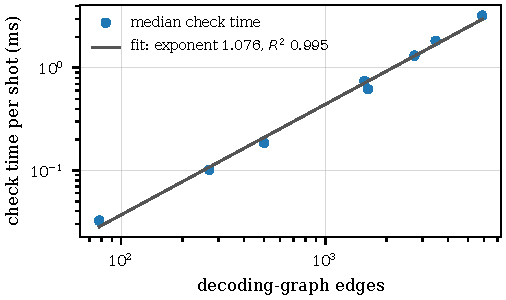
\includegraphics[width=\columnwidth]{figures/checker_scaling.pdf}
\caption{Median time to check one certificate against the number of edges in the decoding graph, with a power-law fit. A first implementation that tested every edge against every dual was close to quadratic; walking set boundaries removed it.}
\label{fig:scaling}
\end{figure}

\paragraph*{Certificates that travel.} A certificate is useful only if a stranger can re-check it, which requires three properties that are easy to lose. It is bound to its graph by a fingerprint the verifier recomputes from its own copy of the graph; otherwise a genuine certificate for an easy instance can be replayed against a hard one with every arithmetic check passing. Every floating-point value travels as its 64-bit pattern, because decimal round-trips differ across languages. And a shot that does not certify still receives a document, labelled not proven, with its gap, so that failure and silence are distinguishable. A signature attests authorship only: a signature over a false certificate is a signed false certificate.

\paragraph*{A second implementation.} A checker written by the same author in the same language cannot expose a shared misreading of the problem. We wrote a second checker in JavaScript from the specification, sharing no code and depending only on the runtime's built-ins. The two agree on all \ConfVectors\ conformance vectors, \ConfRefusals\ of which are refusals, since a suite in which everything verifies would not notice a checker that accepts everything; corrupting one dual value drops the agreement to \ConfVectorsMinusOne. Writing the second checker exposed a genuine ambiguity. Given a packing that listed the same vertex set twice with different values, the Python checker deserialised it into a dictionary, kept the last value, and accepted; the JavaScript checker summed the list, found an edge constraint violated, and refused. One document produced two verdicts. A packing is a map from sets to values, and a list encodes one only while its keys are distinct, so both implementations now refuse a repeated set and the case is a permanent conformance vector. A port of the first implementation would have inherited its reading of the ambiguity; this is why the second was written from the specification.

% ======================================================================
\section{What a receipt proves under floating-point weights}
\label{sec:semantics}

Decoding weights are log-likelihood ratios stored as IEEE-754 doubles, and packings are computed in floating point. Exact equality between a packing's value and $w(J)$ is therefore rarely observable, and a checker must decide what to accept. The choice changes the claim, so we separate two claims:
\begin{itemize}
\item \emph{exact}: $w(J)=\min_{J'} w(J')$ over the double-valued weights, exactly;
\item \emph{$\eps$-optimal}: $w(J)-\min_{J'} w(J')\le\eps$, with $\eps$ proven.
\end{itemize}
Every double is a rational number, so either claim can be decided in exact arithmetic. The following lemma turns any non-negative packing over $\T$-odd sets, feasible or slightly overloaded, into a proven slack.

\begin{lemma}
Let $z\ge0$ be supported on $\T$-odd sets, let $\ell_e=\sum_{S:\,e\in\delt(S)}z_S$, and let $\theta=\min\bigl(1,\min_{e:\,\ell_e>0} w_e/\ell_e\bigr)$. Then $\theta z$ is feasible for~\eqref{eq:packing}, and for every $\T$-join $J$ with minimum $J^\star$,
\[
w(J)-w(J^\star)\;\le\;\eps(J,z)\;:=\;w(J)-\theta\sum_S z_S .
\]
\end{lemma}
\begin{proof}
Each constraint of $\theta z$ reads $\theta\ell_e\le w_e$, which holds by the choice of $\theta$. Applying~\eqref{eq:weakduality} to $\theta z$ and $J^\star$ gives $w(J^\star)\ge\theta\sum_S z_S$.
\end{proof}

\paragraph*{The rule the scale runs used.} The runs in Secs.~\ref{sec:results}--\ref{sec:gaps} were made with a checker that accepted a certificate when its floating-point gap was at most $10^{-6}$ and no edge was overloaded by more than $10^{-9}$. An external audit of this work later showed that any positive tolerance of this kind accepts a correspondingly small suboptimality: a correction of weight $1.0000005$ was accepted against a true optimum of $1$. By the lemma, every certificate accepted under that rule proves $\eps$-optimality with $\eps$ at most about $10^{-6}$, plus a term $10^{-9}\sum_S z_S/\min_e w_e$ that is below \AuditRuleTerm\ on every graph we audited, plus floating-point summation error. Those checkers also lacked a guard against non-finite values, which the same audit found and which was subsequently closed; a NaN in a packing would have been accepted. The reported rates are therefore rates of $\eps$-certification, not of exact certification, and we report them as such.

\paragraph*{The audit.} The full-scale runs did not store their certificates, so their per-shot slack cannot be recovered. To measure what the rule actually certified, we re-ran the exact code that produced each headline artifact, extracted from its commit, on seeded samples of six configurations, kept every certificate it accepted, and analysed each in exact rational arithmetic. Table~\ref{tab:semantics} reports the result. None of the \AuditAccepted\ accepted certificates was inadmissible: all values were finite and non-negative, every set was $\T$-odd, and every correction explained its syndrome. The largest proven slack was \AuditEpsMax. On the three samples from the gap-distribution experiment, the re-run reproduced the artifact's certified counts exactly.

\begin{table*}[tbp]
\caption{Exact re-analysis of the certificates accepted by the code that produced each reported artifact. ``Largest proven slack'' is $\max\eps(J,z)$ from the lemma, computed in rational arithmetic. The last two columns show how today's stricter checker, which demands exact optimality, treats the same certificates, and how many of the same shots today's producer certifies under that stricter rule, using its base ladder and escalation tier but not its exact separation tier, which costs tens of seconds per shot.}
\label{tab:semantics}
\begin{tabular}{@{}lccccc@{}}
\toprule
configuration (code commit) & sample & accepted & largest proven & exact checker, & current producer \\
 & & then & slack $\varepsilon$ & same certificate & (with escalation) \\
\midrule
simulation, $d=5$, 25 rounds (\texttt{d4a81ee}) & 400 & 399 & \ensuremath{1.4\times 10^{-13}} & 54 & 151 \\
simulation, $d=3$, 3 rounds (\texttt{cce1e91}) & 230 & 230 & \ensuremath{2.7\times 10^{-15}} & 213 & 228 \\
simulation, $d=5$, 5 rounds (\texttt{cce1e91}) & 395 & 392 & \ensuremath{1.9\times 10^{-14}} & 339 & 388 \\
simulation, $d=7$, 7 rounds (\texttt{cce1e91}) & 400 & 378 & \ensuremath{7.2\times 10^{-14}} & 124 & 292 \\
Willow, $d=5$, 13 rounds, X (\texttt{06344ae}) & 150 & 149 & \ensuremath{4.7\times 10^{-14}} & 110 & 135 \\
Willow, $d=7$, 30 rounds, X (\texttt{f57e87d}) & 40 & 40 & \ensuremath{2.6\times 10^{-13}} & 2 & 3 \\
\bottomrule
\end{tabular}

\end{table*}

\paragraph*{Exact certification is a different and harder claim.} The checker now in the released code accepts only a proof of exact optimality: it repairs the floating-point rounding of a packing in exact arithmetic and then verifies feasibility and attainment from scratch. It accepts \AuditExactSame\ of the \AuditAccepted\ certificates above (\AuditExactSamePct\%), and the fraction falls steeply with graph size: most of the certificates on small graphs, but few on the 25-round simulation and only a handful on the largest hardware configuration (Table~\ref{tab:semantics}). A consequence must be stated plainly: re-running the reported experiments with the released checker yields certification rates well below those reported, and reproducing the reported rates requires the code at the commits listed in Table~\ref{tab:semantics}. The refusals occur at the scale of the last few bits of a double. On the audited simulation samples, an independent exact-scored matching found PyMatching's correction heavier than an alternative by at most \AuditOracleMaxDelta, and equal on \AuditOracleEqual\ of \AuditOracleN\ shots; that oracle breaks near-ties in floating point, so it cannot settle every case. Because a decoder that computes in floating point is not attempting exact optimality over double-valued weights, and because those weights are estimates far coarser than $10^{-13}$, we regard $\eps$-optimality with a small, proven $\eps$ as the operationally meaningful claim, and report exact certification as a separate, stricter measurement rather than blending the two.

% ======================================================================
\section{Producing the witness}
\label{sec:producer}

Producing a packing is the expensive half. \emph{Moat growth}, Edmonds' primal--dual method~\cite{edmonds1965paths}, grows every $\T$-odd component at equal rate and merges components when an edge becomes tight. It is feasible by construction and \GrowthSpeedupLo--\GrowthSpeedupHi\ times faster than solving a linear program, but at distance~7 it certifies \GrowthDSevenCertified\ shots against \LpDSevenCertified\ for the linear program, because greedy merging picks the wrong pairs.

The main producer solves~\eqref{eq:packing} restricted to a candidate family of sets. Restricting the family cannot cost soundness, since a feasible point of the restricted problem is feasible for the full one; it costs only tightness, which appears as a reported gap. Families of balls around single detectors saturate on long memory experiments, because a ball cannot express a moat around a \emph{group} of detectors. The groups are read from the packing's own slack: a set can carry more value only if every edge on its boundary has slack, so the connected components of the subgraph of tight edges are the sets worth adding. The producer solves, adds those components, and solves again; the objective cannot decrease.

The producer is organised as a ladder whose rungs are tried cheapest first, escalating only on shots the previous rung left open. Generations of the ladder were each introduced against the shots the previous generation could not close: tight-component refinement; sets that cut the correction exactly once, as complementary slackness requires of an optimal dual; candidates translated from the duals of a blossom matching on the metric closure over $\T$; an escalation tier that raises every binding budget on refused shots; and a final exact tier that generates $\T$-odd cuts in the decoding graph by Padberg--Rao separation~\cite{padbergrao1982}, whose converged bound equals the minimum $\T$-join weight. The correction never changes between rungs, and every rung is judged by the same checker, so escalation can tighten a bound but cannot turn a wrong correction into a certified one.

% ======================================================================
\section{Results}
\label{sec:results}

\subsection{Simulation at scale}

We sampled \SimShots\ shots of a distance-5 rotated surface-code memory over 25 rounds at circuit-level depolarising noise $p=0.005$, generated with Stim~\cite{gidney2021stim} and decoded with PyMatching~\cite{higgott2025sparse} on a graph of \SimDetectors\ detectors plus the boundary and \SimEdges\ edges. The ladder $\eps$-certified \SimCertified\ corrections (\SimCertifiedPct\%). Uncertified shots have an $n$-weighted mean gap of \SimGapMean\ and a largest gap of \SimGapMax. The count was completed from a main run and three supplements with disjoint seeds; \SimFailedChunks\ worker chunks (\SimShotsLostToChunks\ shots) died to memory exhaustion at process start or at allocation on a shared workstation. Such deaths occur before or independently of any syndrome's content, so no shot was selected out by difficulty, and the disjoint seeds ensure no shot is counted twice.

\paragraph*{The forgery battery, and why its zero means something.} For every shot, certified or not, we built forged certificates from the strongest packing found, in seven classes: corrections with a dropped, duplicated, or mismatched edge; strictly heavier corrections; corrections with a spurious cycle; a heavier correction with the packing scaled to meet its weight; and the same with a negative value hiding the inflation. Of \SimForgeries\ forgeries, \SimForgeriesAccepted\ were accepted. Twice during development an ``attack'' was accepted and the checker was right: once the forged correction was an equal-weight alternative optimum, and once a construction meant to hide a negative value degenerated into a valid certificate for an optimal correction. Both were attacks whose claim happened to be true. Every forgery is therefore re-verified to be false, independently of the checker, before its verdict is counted, and a run in which any forgery fails that test is void. The battery did not include non-finite values or substituted graphs; those cases are covered by the checker's own tests rather than by these counts.

\subsection{Google Willow}

We applied the same producer and checker to detector samples from Google's Willow processor~\cite{google2025below,google2024data}, decoded on the error models the experimenters published with the data, so the weights are not ours to choose. Table~\ref{tab:generations} gives the certified rate for the first four producer generations, each measured against the shots its predecessor left open; these rates were committed to before the next generation existed. The first generation certified \HwGenOnePct\% of \HwGenOneNontrivial\ nontrivial shots, far below the simulated rate. Coverage differed between generations: generations 2 and 3 ran partial samples, down to \HwGenTwoMinConfig\ shots for one configuration, so their aggregates weight configurations unequally. Generation 4 ran every configuration at 10{,}000 shots, with no shot lost to infrastructure.

\begin{table*}[tbp]
\caption{Certified percentage on Willow shots, X / Z basis, by producer generation. Generation 1 ran 50{,}000 shots per configuration; generations 2 and 3 ran partial coverage; generation 4 ran 10{,}000 per configuration. Each value is computed from the artifact that generation wrote, including the two generations whose artifacts survive only in version history.}
\label{tab:generations}
\begin{tabular}{@{}lcccc@{}}
\toprule
configuration & gen.~1 & gen.~2 & gen.~3 & gen.~4 \\
\midrule
$d=3$, 13 rounds & 96.19 / 96.65 & 99.16 / 99.39 & 99.99 / 99.98 & 100.00 / 100.00 \\
$d=3$, 30 rounds & 89.62 / 89.84 & 98.79 / 98.97 & 99.98 / 99.97 & 100.00 / 99.99 \\
$d=5$, 13 rounds & 88.22 / 89.31 & 95.86 / 96.37 & 98.71 / 98.92 & 99.67 / 99.72 \\
$d=5$, 30 rounds & 67.68 / 69.67 & 89.40 / 89.49 & 95.86 / 95.85 & 98.75 / 98.96 \\
$d=7$, 13 rounds & 78.46 / 78.53 & 90.67 / 90.58 & 95.40 / 95.63 & 98.30 / 98.49 \\
$d=7$, 30 rounds & 49.02 / 49.30 & 73.62 / 76.48 & 84.80 / 86.45 & 93.76 / 94.71 \\
\midrule
aggregate & 78.44 & 93.09 & 96.04 & 98.52 \\
nontrivial shots & 596{,}732 & 107{,}184 & 117{,}235 & 119{,}384 \\
per configuration & 47{,}631--50{,}000 & 800--10{,}000 & 9{,}300--10{,}000 & 9{,}560--10{,}000 \\
\bottomrule
\end{tabular}

\end{table*}

The two hardest configurations, distance 7 over 30 rounds, were re-run at 50{,}000 shots per basis, first with the escalation tier (\HwGenFiveXPct\% and \HwGenFiveZPct\%) and then with the exact tier added. With the exact tier, \HwGenSixXCertified\ of \HwGenSixXNontrivial\ shots were certified in each basis (\HwGenSixXPct\%), with \HwGenSixXExactRung\ (X) and \HwGenSixZExactRung\ (Z) shots reaching the exact tier and one shot per basis left uncertified, at gaps \HwGenSixXResidualGap\ and \HwGenSixZResidualGap. Certification cost \HwCoreSecX\ s (X) and \HwCoreSecZ\ s (Z) of core time per shot, or \HwWallSecX\ s and \HwWallSecZ\ s of wall time. Counting each configuration at its final generation, \HwFinalCertified\ of \HwFinalNontrivial\ hardware shots were certified (\HwFinalPct\%), and none of \HwForgeries\ forgeries was accepted. Fig.~\ref{fig:ladder} shows the uncertified fraction per configuration across generations.

\begin{figure}[tbp]
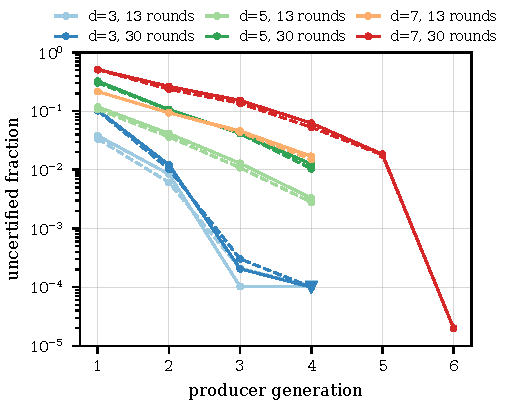
\includegraphics[width=\columnwidth]{figures/generation_ladder.pdf}
\caption{Uncertified fraction per Willow configuration by producer generation; solid lines X basis, dashed Z. Generations 5 and 6 re-ran only distance 7 over 30 rounds. Where no shot was left uncertified, the point is drawn at $1/n$.}
\label{fig:ladder}
\end{figure}

\subsection{Is the decoder, or the producer, responsible for refusals?}
\label{sec:oracle}

A refusal can mean the decoder's correction was not optimal or that the producer failed to find a tight packing. To separate the two we computed, for every nontrivial shot of three simulated configurations, a minimum-weight perfect matching on the metric closure over $\T$ with per-detector boundary copies, using networkx~\cite{hagberg2008networkx}: a different formulation and algorithm, sharing no code with the producer. On all \OracleShots\ shots (\OracleShotsThree\ at distance 3 over \OracleRoundsThree\ rounds, \OracleShotsFive\ at distance 5 and \OracleShotsSeven\ at distance 7, both over 25 rounds) the oracle's weight equalled the decoder's, so every refusal on those shots was producer slack. The oracle breaks near-ties in floating point, so this agreement holds to floating-point resolution, which is the same resolution as the $\eps$-claim.

\subsection{Other hardware}

To check that nothing is specific to one vendor's data format or graph construction, we certified a repetition-code memory run on IBM's \IbmBackend\ processor, preregistered before submission (SHA-256 prefix \texttt{\IbmPreregPrefix}): all \IbmCertified\ of \IbmNontrivial\ nontrivial shots were certified, at \IbmMsPerShot\ ms per shot. Here the error model is ours, a declared uniform model, not the experimenters', and the forgery battery was not run, so these shots are reported separately from every total above.

% ======================================================================
\section{What the certificate detects}
\label{sec:detection}

\subsection{Seeded decoder faults}

We mutated the decoder's output at distances 3, 5 and 7 with defects of several kinds, which models wrong answers but not crashes, hangs, or memory errors. Across all \FaultsAll\ defective corrections, syndrome consistency detected \FaultsAllSyndromeCaught\ (\FaultsAllSyndromePct\%) and the certificate all \FaultsAllCertCaught. The informative subset is the \FaultsStealth\ faults constructed to leave the syndrome exactly satisfied while making the correction strictly heavier: syndrome consistency detected \FaultsStealthSyndromeCaught\ and the certificate \FaultsStealthCertCaught. As a negative control, \FaultsControl\ equal-weight alternative optima (generated at distances 3 and 5; none arose at distance 7) were flagged \FaultsControlFlagged\ times. The full corpus of \FaultCorpus\ seeded cases is released so other detectors can be scored on the same faults.

This experiment is open to the objection that the mutations were chosen knowing what the certificate checks. The next one is not.

\subsection{A stale calibration}

Here the decoder runs unmodified and its output is never touched. The fault is upstream: the decoder decodes on a graph built from a drifted error model, as it would if its calibration snapshot were stale, and its corrections are checked against the true graph. Stale snapshots arise when calibration jobs fail and the previous snapshot is reused, or when a deployment points at the wrong run. Every correction is syndrome-consistent by construction, because the decoder solves a correct problem with wrong weights.

\begin{table}[!tbp]
\caption{Stale-calibration fault at drift factor 3.0. Every correction in every row is syndrome-consistent; ``suboptimal'' counts corrections strictly heavier than optimal under the true weights.}
\label{tab:stale}
\small\setlength{\tabcolsep}{3.5pt}
\begin{tabular}{@{}lcccccc@{}}
\toprule
 & & proven & false & \multicolumn{3}{c}{logical errors} \\
 & $N$ & subopt. & alarms & stale only & ref.\ only & both \\
\midrule
$d=3$ & 452 & 24 & 0 & 1 & 1 & 6 \\
$d=5$ & 797 & 76 & 0 & 4 & 0 & 12 \\
$d=7$ & 800 & 171 & 0 & 3 & 1 & 4 \\
\bottomrule
\end{tabular}

\end{table}

Table~\ref{tab:stale} shows drift factor 3.0. Across the drift factors 1.5, 2.0 and 3.0, the stale decoder produced \StaleSuboptimalOneFive, \StaleSuboptimalTwo\ and \StaleSuboptimalThree\ suboptimal corrections; syndrome checking detected \StaleSyndromeCaughtTotal\ of the \StaleSuboptimalTotal\ and the certificate \StaleCertCaughtTotal. What scales with drift is severity, not detectability: the mean excess weight rises from \StaleExcessLoOneFive--\StaleExcessHiOneFive\ at drift 1.5 to \StaleExcessLoThree--\StaleExcessHiThree\ at drift 3.0 across distances. At distance 3 and drift 3.0, the logical error count is \StaleDThreeLogicalTrue\ under both the true and the stale model while \StaleDThreeSuboptimal\ corrections are suboptimal, so the logical error rate, the measurement the field relies on, carries no signal. As a control, drift factor 1.0 produced \StaleControlSuboptimal\ suboptimal corrections at every distance; a nonzero count there would mean the harness manufactures defects.

% ======================================================================
\section{Per-shot optimality gaps}
\label{sec:gaps}

Decoders are usually compared by logical error rate, an average that cannot distinguish a decoder that is consistently slightly suboptimal from one that is usually exact with a heavy tail. A certified optimum on the same shot makes the individual gap measurable. Restricting to shots whose minimum-weight correction was certified, the bound equals the optimum and each decoder's gap is its excess weight. We sampled \GapShotsPerDistance\ shots per distance with rounds equal to distance at $p=0.005$ and decoded each with BP-OSD~\cite{panteleev2021degenerate,roffe2020decoding} and belief-matching~\cite{higgott2023improved}; Table~\ref{tab:gaps} reports BP-OSD.

\begin{table}[tbp]
\caption{BP-OSD's excess weight over the certified minimum, on shots whose minimum-weight correction was $\eps$-certified.}
\label{tab:gaps}
\small\setlength{\tabcolsep}{3.5pt}
\begin{tabular}{@{}lccccc@{}}
\toprule
 & certified & BP-OSD & \multicolumn{3}{c}{gap} \\
 & shots & exact & median & p99 & max \\
\midrule
$d=3$ & 230 & 81.3\% & 0.0 & 38.1 & 68.0 \\
$d=5$ & 392 & 72.7\% & 0.0 & 60.8 & 148.0 \\
$d=7$ & 378 & 74.3\% & 0.0 & 52.2 & 78.7 \\
\bottomrule
\end{tabular}

\end{table}

BP-OSD lands exactly on the certified minimum on most shots and, when it departs, departs by up to \GapBposdMax\ weight units. A gap is not a defect: BP-OSD maximises likelihood over the full hypergraph, where the minimum-weight $\T$-join of the decomposed graph is not the maximum-likelihood answer, and weight is not homology class. The reading is distributional. Belief-matching optimises under weights informed by belief propagation, so it too is not attempting minimum weight under the original weights, yet it lands far closer: its 99th-percentile gap is \GapBmPNinetyNine\ at distances 3, 5 and 7 against \GapBposdPNinetyNine\ for BP-OSD. Repeating the experiment with the exact checker certifies \GapExactRuleCertified\ of the same shots, and BP-OSD is exact on \GapExactRuleBposdExact\%; the conclusion is unchanged. Fig.~\ref{fig:gaps} shows the tails.

\begin{figure}[tbp]
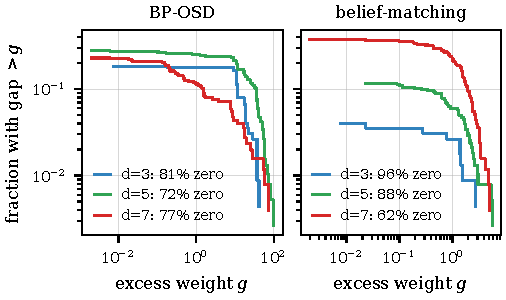
\includegraphics[width=\columnwidth]{figures/gap_tails.pdf}
\caption{Fraction of shots whose excess weight over the certified minimum exceeds $g$, on shots the exact checker certified. The remaining mass sits at exactly zero; the legend gives its size.}
\label{fig:gaps}
\end{figure}

% ======================================================================
\section{Cost}
\label{sec:cost}

On the distance-5, 25-round graph, certification cost \CertifyMsPerShot\ ms per shot against about \DecodeUsBatch~$\mu$s per shot for batch decoding and \DecodeUsPerShot~$\mu$s for per-shot decoding, measured on the same graph: ratios of \CostRatioBatch\ and \CostRatioPerShot. That excludes certification from the real-time decoding loop with current producers and suits offline audit, acceptance testing of decoder releases, and spot-checking a sampled fraction of a live stream. Checking a certificate, as opposed to producing one, is cheap (Fig.~\ref{fig:scaling}).

% ======================================================================
\section{Related work and scope}
\label{sec:related}

\paragraph*{Certifying and checking.} Certifying algorithms~\cite{mcconnell2011certifying} and program checkers~\cite{blumkannan1995} are classical, as is the linear-programming structure of matching and $\T$-joins~\cite{edmonds1965polyhedron,edmondsjohnson1973}. In exact integer programming, the gap between a floating-point solver's claim and a proof is well studied, with safe dual bounds and verifiable certificates~\cite{steffy2013valid,cheung2017verifying,eifler2023computational}; Sec.~\ref{sec:semantics} addresses the same issue for decoding receipts.

\paragraph*{Decoding.} Wu \textit{et al.}~\cite{wu2025minimum} formulate most-likely-error decoding as a minimum-weight parity factor problem with a primal--dual model and certifiable proximity bounds, so the observation that decoding has a checkable dual is not new. This paper's contribution is the assurance engineering and measurement around it. Linear-programming decoding of classical and quantum codes has a long history~\cite{feldman2005lp,li2018lp}.

\paragraph*{Concurrent work.} Three recent preprints sit close to this one. Krishnamoorthy \textit{et al.}~\cite{krishnamoorthy2026certified} certify decoding decisions on surface and bivariate-bicycle codes, including exact maximum-likelihood decoding on tested surface-code instances; their object is degenerate-coset maximum likelihood and their certificates are internal to a sampler, whereas the receipts here are re-checkable by a third party from the syndrome and graph alone. Shen and Zhong~\cite{shen2026capability} test decoder libraries for conformance with a standalone verifier, the same verifier-side posture aimed at libraries rather than individual shots. Ehatamm \textit{et al.}~\cite{ehatamm2026end} formalise quantum error correction end to end in a proof assistant, verifying the framework rather than individual instances. Our literature searches, whose queries are logged with the released artifacts, did not find the forgery battery, the upstream-fault detection experiment, or hardware certification rates elsewhere; not finding them is not proof of absence.

\paragraph*{What is not claimed.} Certification is not a real-time decoder (Sec.~\ref{sec:cost}). It is not complete: \SimUncertifiedPct\% of simulated shots and one shot per basis in the hardest hardware configuration were not certified, and those receive receipts stating a measured gap. The rates are properties of our producer, a decoder, and an error model; soundness is a property of the checker alone. The reported rates are $\eps$-certification rates in the sense of Sec.~\ref{sec:semantics}. A certificate proves optimality for the weights it was given, and says nothing about whether those weights describe the device.

% ======================================================================
\section{Reproducibility and data}
\label{sec:repro}

Code, artifacts, conformance vectors, the seeded-fault corpus and the certificate schema are released under the Apache License 2.0 at \url{https://github.com/coherence-energy-labs/oneq-certificates}. Every number in this paper is typeset from a macro generated from a JSON artifact, and each artifact records the command and code that produced it; the certification-semantics audit (Table~\ref{tab:semantics}) re-runs the producing code of each headline artifact from its commit. The Willow data are read in place from the published archive~\cite{google2024data}. Validating a certificate against its schema establishes only that it is well formed; establishing that its claim is true requires re-running a checker against a graph the verifier supplies.

\paragraph*{Use of AI tools.} AI tools assisted with software development and manuscript preparation; the author is responsible for all content.

\bibliography{refs}

\end{document}
